\subsection{Schritt 1: Gaussian Blur}
\label{sec:impl_gaussian}

\subsubsection{Naive Implementierung}

Die Gaußgewichte werden auf der CPU vorberechnet und normalisiert
(Summe~1, Gleichung~\ref{eq:gaussian}), einmalig per \texttt{cudaMemcpy}
auf die GPU übertragen und stehen dort als Read-only-Buffer im globalen
Speicher zur Verfügung. Abbildung~\ref{fig:gaussian_example} zeigt das
resultierende $3 \times 3$ Gewichtsraster für $\sigma = 1.0$.

\begin{figure}[H]
    \centering
    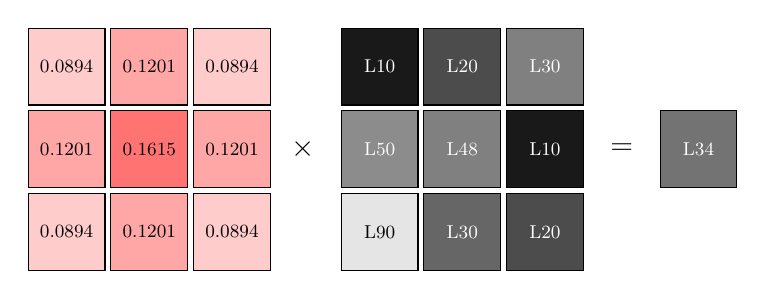
\begin{tikzpicture}[
        scale=0.75,
        every node/.style={transform shape},
        pixel/.style={rectangle, draw, minimum size=1.3cm, align=center, font=\small, inner sep=2pt},
        k_low/.style={pixel,  fill=red!20},
        k_mid/.style={pixel,  fill=red!35},
        k_high/.style={pixel, fill=red!55}
    ]

        \node[k_low]  at (0,0)      {0.0894};
        \node[k_mid]  at (1.4,0)    {0.1201};
        \node[k_low]  at (2.8,0)    {0.0894};
        \node[k_mid]  at (0,-1.4)   {0.1201};
        \node[k_high] at (1.4,-1.4) {0.1615};
        \node[k_mid]  at (2.8,-1.4) {0.1201};
        \node[k_low]  at (0,-2.8)   {0.0894};
        \node[k_mid]  at (1.4,-2.8) {0.1201};
        \node[k_low]  at (2.8,-2.8) {0.0894};

        \node[font=\Large] at (4.0,-1.4) {$\times$};

        \node[pixel, fill=black!90, text=white] at (5.3,0)    {L10};
        \node[pixel, fill=black!70, text=white] at (6.7,0)    {L20};
        \node[pixel, fill=black!50, text=white] at (8.1,0)    {L30};
        \node[pixel, fill=black!45, text=white] at (5.3,-1.4) {L50};
        \node[pixel, fill=black!50, text=white] at (6.7,-1.4) {L48};
        \node[pixel, fill=black!90, text=white] at (8.1,-1.4) {L10};
        \node[pixel, fill=black!10]             at (5.3,-2.8) {L90};
        \node[pixel, fill=black!60, text=white] at (6.7,-2.8) {L30};
        \node[pixel, fill=black!70, text=white] at (8.1,-2.8) {L20};

        \node[font=\Large] at (9.4,-1.4) {$=$};

        \node[pixel, fill=black!55, text=white] at (10.7,-1.4) {L34};

    \end{tikzpicture}
    \caption{Gaussian Blur, gewichteter Mittelwert am Beispielpixel L48 $\rightarrow$ L34}
    \label{fig:gaussian_example}
\end{figure}

Im CUDA-Kernel \texttt{gaussian\_filter()} ist jeder Thread für genau
einen Ausgabepixel zuständig; Threads außerhalb der Bildgrenzen werden
sofort verworfen. Jeder Thread iteriert über alle $(2r+1)^2$
Nachbarpixel, liest jeden Wert direkt aus dem globalen Speicher und
akkumuliert die gewichtete Summe, wobei Pixel außerhalb der
Bildgrenzen mit~0 aufgefüllt werden (Zero-Padding). Die Threads eines
Blocks greifen dabei in y-Richtung auf Adressen mit Abstand
\texttt{width} zu, wodurch die Zugriffe auf den globalen Speicher nicht
coalesced erfolgen, was die in Abschnitt~\ref{sec:shared_memory_gaussian}
beschriebene Shared Memory Optimierung motiviert; die quantitative
Auswertung findet sich in Abschnitt~\ref{sec:results_gaussian}.

\subsubsection{Shared Memory Optimierung}
\label{sec:shared_memory_gaussian}

Bei einem Kernel der Größe $(2r+1)^2$ liest jeder Thread bis zu
$(2r+1)^2$ Pixel redundant aus dem DRAM. \cite[S.~2]{horvath2023}
adressieren dieses Problem durch Shared Memory Tiling, bei dem Threads
eines Blocks kooperativ eine Bildkachel inklusive Halo-Rand der Größe
$(\texttt{BLOCK\_SIZE} + 2 \cdot \texttt{BLUR\_RADIUS})^2$ in den
On-Chip Speicher laden, bevor \texttt{\_\_syncthreads()} die
vollständige Ladephase sicherstellt. Die Gaußgewichte werden zusätzlich
in \texttt{\_\_constant\_\_} Memory ausgelagert, da alle Threads
dieselben Gewichte lesen und dieser Speicher für uniforme Zugriffe
hardwareseitig gecacht wird. Die Auswirkung dieser Optimierung auf
Laufzeit und Speicherdurchsatz wird in
Abschnitt~\ref{sec:results_gaussian} ausgewertet.

\subsubsection{Pinned Memory Optimierung}
\label{sec:pinned_memory_gaussian}

Pinned Memory (Page-locked Memory) ist Host-seitiger Speicher, der vom
Betriebssystem nicht ausgelagert werden kann, wodurch direkte
DMA-Transfers ohne zwischengeschalteten CPU-Cache möglich sind. Die
Änderung gegenüber der Shared Memory Implementierung beschränkt sich
auf die Host-seitige Allokation (\texttt{cudaMallocHost()} statt
\texttt{malloc()}); der Kernel bleibt identisch, der erwartete Vorteil
zeigt sich primär beim Device-to-Host-Transfer
(Abschnitt~\ref{sec:results_gaussian}).

\subsubsection{Warp-Level Optimierung}

Als vierte Stufe wurden Warp-Level Intrinsics
(\texttt{\_\_shfl\_sync()}) evaluiert, die Datenaustausch innerhalb
eines Warps ohne Shared Memory ermöglichen. Für 2D-Stencil-Operationen
wie den Gaussian Blur ist dieser Ansatz jedoch ungeeignet, da
\texttt{\_\_shfl\_sync()} primär für 1D-Reduktionen konzipiert ist, was
\cite{yadav2025} bestätigen (79.29\,\% vs.\ 83.33\,\% Compute/Memory
Throughput bei Shared Memory). Eine eigene Implementierung wurde daher
nicht vorgenommen.